\documentclass{beamer}
\usepackage[utf8]{inputenc}
\usepackage{amsmath, amssymb, amsthm}
\usepackage{tikz}
\usepackage{listings}

\usetheme{CambridgeUS}
\usecolortheme{crane}

\title{From Abstraction to Computation: \\ Understanding Lambda Calculus}
\author{Pratham Gupta Sehaj Ganjoo\\
        Krishna Agarwal Gavish Bansal}
\institute{Indian Institute of Science, Bengaluru}
\date{\today}

\AtBeginSection[]
{
  \begin{frame}[allowframebreaks]
    \frametitle{Outline}
    \tableofcontents[currentsection]
  \end{frame}
}

% \AtBeginSubsection[]
% {
%   \begin{frame}[allowframebreaks]
%     \frametitle{Outline}
%     \tableofcontents[currentsection,currentsubsection]
%   \end{frame}
% }


\begin{document}

% Slide 1: Title Slide
\begin{frame}
  \titlepage
\end{frame}

% Slide 2: Outline
\begin{frame}{Outline}
  \tableofcontents
\end{frame}

% Section 1: Introduction and Motivation
\section{Introduction and Motivation}

\begin{frame}{Historical Background}
\textbf{Leibniz’s Ideal:}
\begin{itemize}
    \item A "universal language" to express all possible problems.
    \item A decision method to solve all problems in this language.
\end{itemize}
\bigskip
By the early 20th century, set theory and first-order logic (Frege, Russell, Zermelo) fulfilled point (1).\\
However, point (2) remained open—this became the Entscheidungsproblem ("decision problem"):\\
\begin{quote}
    Can all problems be solved mechanically?
\end{quote}
\end{frame}
\begin{frame}{Historical Background}
Alonzo Church and Alan Turing independently proved that no general algorithm can decide the truth of all mathematical statements.\\
In order to do so, they had to formalize "computability.\\
\begin{itemize}
    \item Church (1936): Introduced lambda calculus as a formal model of computation
    \item Turing (1936/37): Introduced Turing machines as an alternative model.
    \item Turing (1937): Proved both models are equivalent—defining the same class of computable functions
\end{itemize}

\end{frame}
%Hilbert’s Entscheidungsproblem (1928):
% (“decision problem”)
% Given a sentence in first-order logic, give an “effectively calculable procedure” for determining if it’s provable.
% Mathematicians: “we should probably try to formalize what counts as an ‘algorithm’ ”.
% \begin{frame}{Historical Background}
%   \begin{itemize}
%     \item Developed by Alonzo Church in the 1930s.
%     \item Originally intended as a foundation for mathematics.
%     \item Inspired by higher-order logic and the concept of functions.
%     \item Later became a model of computation equivalent to Turing machines.
%   \end{itemize}
% \end{frame}

\begin{frame}{Motivation}
  \begin{itemize}
    \item Addressing Russell’s paradox in set theory.
    \item Establishing a formal system for computability.
    \item Laying the groundwork for functional programming languages.
  \end{itemize}
\end{frame}

\begin{frame}{Church-Turing Thesis}
Any natural / reasonable notion of computation realizable in the physical world can be simulated by a TM (or equivalently, by lambda calculus)
\end{frame}

\begin{frame}{Overview of Topics}
  \begin{itemize}
    \item Syntax of the lambda-calculus.
    \item Free and bound variables.
    \item Substitution and $\alpha$-conversion.
    \item $\beta$-reduction and the Church–Rosser theorem.
    \item Combinators and representation of booleans.
    \item Encoding natural numbers.
    \item Fixed-point combinators and recursion.
    \item $\lambda$-definability of computable functions.
  \end{itemize}
\end{frame}

% Section 2: Syntax of the Lambda Calculus
\section{Syntax of the Lambda Calculus}
\begin{frame}{Basic Concepts}
  \begin{itemize}
    \item \textbf{Variables:} $x, y, z, \dots$
    \item \textbf{Abstraction:} $\lambda x.M$ (function definition)
    \item \textbf{Application:} $(MN)$ (function application)
  \end{itemize}
\end{frame}

\subsection{$\lambda$-Terms}
\begin{frame}{Formal Definition of $\lambda$-Terms}
  \begin{block}{Definition}
    The set of $\lambda$-terms is defined inductively:
    \begin{enumerate}
      \item Any variable $x$ is a $\lambda$-term.
      \item If $M$ and $N$ are $\lambda$-terms, then $(M N)$ is a $\lambda$-term called an \textbf{application}
      \item If $M$ is a $\lambda$-term and $x$ is a variable, then $\lambda x.M$ is a $\lambda$-term called a $\lambda$-abstraction
    \end{enumerate}
  \end{block}
  \textbf{Examples:}
  \begin{itemize}
      \item let $M = \lambda x.x$ is a lambda abstraction 
      \item let $N = y $
      \item $(M N) = (\lambda x.x \; y) \rightarrow y$
  \end{itemize}
\end{frame}

\begin{frame}{Formal Definition of $\lambda$-Terms}
  \begin{block}{Some Valid Lambda Expressions:}
  \begin{itemize}
      \item $x$
      \item $\lambda x.x$
      \item $xy$
      \item x$\lambda$ y.$(x(yy))$
      \item $\lambda\lambda x.y$ (invalid)
  \end{itemize}
  \end{block}
\end{frame}

\begin{frame}{Tree Representation}
    \begin{itemize}
      \item Each $\lambda$-term can be represented as a labeled tree.
      \item Leaves represent variables.
      \item Interior nodes represent applications or abstractions.
    \end{itemize}
    \begin{center}
      % Replace with your own image if desired
        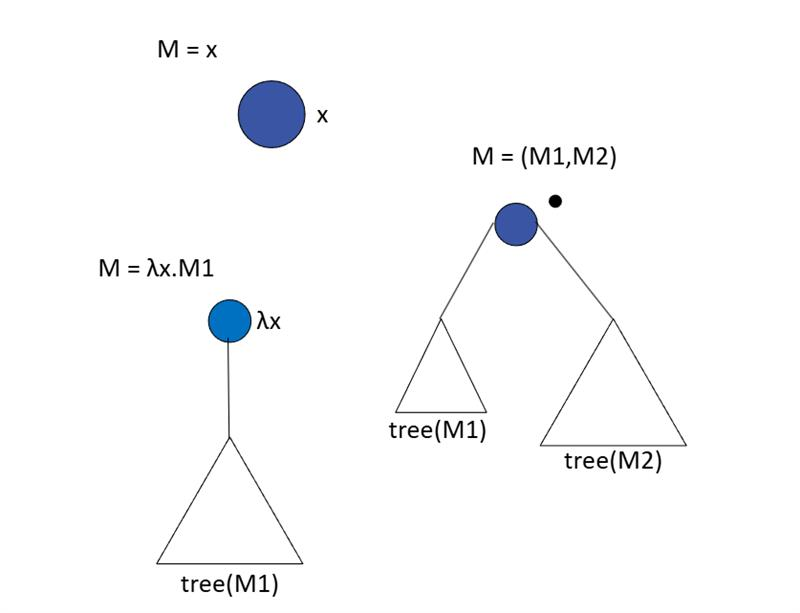
\includegraphics[width=0.5\textwidth]{images/treeimage.png}
    \end{center}
\end{frame}
  


\begin{frame}{Notation Conventions}
  \begin{itemize}
    \item Left-association of application:
      \[
        (((F \; M_1)M_2)\ldots M_n) \quad\text{is written as}\quad F M_1 \ldots M_n.
      \]
    \item Right-association of abstractions:
      \[
        \lambda x_1.\lambda x_2.\cdots\lambda x_n.M \quad\text{is written as}\quad \lambda x_1 \cdots x_n.M.
      \]
  \end{itemize}
\end{frame}


\subsection{Free and Bound Variables}
\begin{frame}{Free vs. Bound Variables}

  \begin{definition}
    For any $\lambda$-term \(M\), the \textbf{free variables} (FV) and \textbf{bound variables} (BV) are defined as follows:
    \begin{itemize}
      \item If $M = x$ is a variable, then:
        \[
        \text{FV}(x) = \{x\}, \quad \text{BV}(x) = \emptyset
        \]
      \item If $M = (M_1 M_2)$, then:
        \[
        \text{FV}(M) = \text{FV}(M_1) \cup \text{FV}(M_2), \quad \text{BV}(M) = \text{BV}(M_1) \cup \text{BV}(M_2)
        \]
      \item If $M = \lambda x.M_1$, then:
        \[
        \text{FV}(M) = \text{FV}(M_1) \setminus \{x\}, \quad \text{BV}(M) = \text{BV}(M_1) \cup \{x\}
        \]
    \end{itemize}
  \end{definition}



\end{frame}

\begin{frame}{Free and Bound Variables}

  \begin{definition}
    A $\lambda$-term M is closed or a \textbf{Combinator} if it has no free variables, i.e., $\text{FV}(M) = \emptyset$.
  \end{definition}

  Intuitively:
  \begin{itemize}
    \item \textbf{Free Variables (FV):} Occur unbound in a term.
    \item \textbf{Bound Variables (BV):} Declared within a $\lambda$-abstraction.
  \end{itemize}
  \vspace{1em}
  \[
  \text{For } M_1 = \lambda x. (xy), \quad \text{FV}(M_1)=\{y\},\quad \text{BV}(M_1)=\{x\}.
  \]
  \[
  \text{For } M_2 = \lambda x.(\lambda y. (x)), \quad \text{FV}(M_2)=\emptyset,\quad \text{BV}(M_2)=\{x,y\}.
  \]
  Note that:
  \begin{itemize}
    \item \(M_2\) has no free variables and is a combinator.
    \item If we rename a bound variable in a term, It has no effect on the behavior of the term.
  \end{itemize}
\end{frame}


% Section 4: Substitution and Alpha-Conversion
\section{Substitution and $\alpha$-Conversion}
\begin{frame}{Substitution}
  \begin{itemize}
    \item Replacing all free occurrences of a variable \(x\) in \(M\) by a term \(N\).
    \item Notation: \(M[x := N]\).
    \item Must avoid variable capture.
  \end{itemize}
\end{frame}

% \begin{frame}{Example of Substitution}
%   \[
%     (\lambda x. (xz)(yz))[y := (vv)] \rightarrow \lambda x.\Bigl(x(λu.v) \Bigr)\Bigl((vv)(λu.v)\Bigr)
%   \]
%   \vspace{0.5em}
%   \begin{itemize}
%     \item Illustrates careful handling to avoid capture.
%   \end{itemize}
% \end{frame}

\begin{frame}{$\alpha$-Conversion}
  \begin{itemize}
    \item Renaming bound variables to avoid clashes.
    \item \(\lambda x.M \equiv \lambda y.M[x:=y]\) provided \(y \notin FV(M)\).
    \item Essential for correct substitution.
  \end{itemize}
\end{frame}

% Section 5: Beta-Reduction and Church–Rosser
\section{Beta-Reduction and Church–Rosser}
\begin{frame}{Beta-Reduction}
  \begin{block}{Definition}
    \[
    (\lambda x.M)N \rightarrow_\beta M[x:=N]
    \]
    \begin{itemize}
      \item The fundamental rule of computation.
    \end{itemize}
  \end{block}
\end{frame}

\begin{frame}{Examples of $\beta$-Reduction}
  \begin{itemize}
    \item \((\lambda xy.x)uv \rightarrow_\beta u\).
    \item \((\lambda xy.y)uv \rightarrow_\beta v\).
  \end{itemize}
\end{frame}

\begin{frame}{Church–Rosser Theorem}
  \begin{itemize}
    \item Confluence: If \( M \) reduces to both \( M_1 \) and \( M_2 \), then there exists \( M_3 \) such that both \( M_1 \) and \( M_2 \) reduce to \( M_3 \).
    \item Implies uniqueness (up to $\alpha$-conversion) of normal forms.
  \end{itemize}
\end{frame}

% Section 6: Useful Combinators
\section{Some Useful Combinators}
\begin{frame}{Combinators I, K, and S}
  \begin{itemize}
    \item \( I = \lambda x.x \)
    \item \( K = \lambda xy.x \)
    \item \( S = \lambda xyz. (xz)(yz) \)
  \end{itemize}
  \vspace{1em}
  \[
    SKK \rightarrow_\beta I
  \]
\end{frame}

\begin{frame}{Additional Combinators}
  \begin{itemize}
    \item \( K^* = \lambda xy.y \)
    \item Booleans: \(T = K\) and \(F = K^*\)
    \item Conditional: \(\text{if} = \lambda bxy. bxy\)
  \end{itemize}
\end{frame}

\begin{frame}{Pairs and Projections}
  \begin{itemize}
    \item Pair: \(\langle M, N \rangle = \lambda z. zMN\)
    \item First projection: \(\pi_1 = \lambda z. zK\)
    \item Second projection: \(\pi_2 = \lambda z. zK^*\)
  \end{itemize}
\end{frame}

% Section 7: Representing Natural Numbers
\section{Representing Natural Numbers}
\begin{frame}{Church Numerals}
  \begin{block}{Definition}
    \[
    c_n = \lambda f x. f^n(x)
    \]
    \begin{itemize}
      \item \(c_0 = \lambda f x. x\)
      \item \(c_1 = \lambda f x. f x\), \(c_2 = \lambda f x. f (f x)\), etc.
    \end{itemize}
  \end{block}
\end{frame}

\begin{frame}{Iteration with Church Numerals}
  \[
    \text{Iter} = \lambda nfx. n f x
  \]
  \begin{itemize}
    \item Iterates the function \(f\) \(n\) times on \(x\).
  \end{itemize}
\end{frame}

\begin{frame}{Arithmetic Operations}
  \begin{itemize}
    \item \textbf{Addition:} \( \text{Add} = \lambda m n f x. m f (n f x) \)
    \item \textbf{Multiplication:} \( \text{Mult} = \lambda m n. m n \)
  \end{itemize}
\end{frame}

\begin{frame}{The Predecessor Function}
  \begin{itemize}
    \item More challenging to define.
    \item Kleene’s solution uses pairs:
      \[
      \text{Pred} = \lambda n. \pi_2 \Bigl( \text{Iter}\ n\ \bigl(\lambda z. \langle \text{Succ}(\pi_1 z),\pi_1 z \rangle\bigr)\ \langle c_0, c_0 \rangle \Bigr)
      \]
  \end{itemize}
\end{frame}

\begin{frame}{Barendregt Numerals}
  \begin{itemize}
    \item Alternative representation: 
      \[
      b_0 = I,\quad b_{n+1} = \langle F, b_n \rangle
      \]
    \item Simpler for certain arithmetic operations.
  \end{itemize}
\end{frame}

% Section 8: Fixed-Point Combinators and Recursion
\section{Fixed-Point Combinators and Recursion}
\begin{frame}{Fixed-Point Combinators}
  \begin{itemize}
    \item Enable recursive definitions without explicit recursion.
    \item \textbf{Curry's Y-combinator:}
      \[
      Y = \lambda f. (\lambda x. f (x x)) (\lambda x. f (x x))
      \]
  \end{itemize}
\end{frame}

\begin{frame}{Properties of the Y-Combinator}
  \begin{itemize}
    \item For any \(F\), \(F (Y F) \equiv_\beta Y F\).
    \item Note: Reduction may not go both ways directly.
  \end{itemize}
\end{frame}

\begin{frame}{Turing's $\Theta$-Combinator}
  \begin{itemize}
    \item Defined as:
      \[
      \Theta = (\lambda x y. y(x x y)) (\lambda x y. y(x x y))
      \]
    \item Satisfies:
      \[
      \Theta F \rightarrow_\beta F (\Theta F)
      \]
  \end{itemize}
\end{frame}

\begin{frame}{Defining Recursive Functions}
  \begin{itemize}
    \item To define a recursive function \(G\) such that
      \[
      G X \rightarrow_\beta M(X, G)
      \]
    \item Let \(F = \lambda g x. M(x, g)\) and define \(G = \Theta F\).
  \end{itemize}
\end{frame}

\begin{frame}{Example: Factorial Function}
  \begin{itemize}
    \item Define:
      \[
      F = \lambda g n.\, \text{if}\ (\text{IsZero}\ n)\ \text{then}\ c_1\ \text{else}\ \text{Mult}\ n\ (g\ (\text{Pred}\ n))
      \]
    \item Then \(G = \Theta F\) represents the factorial function.
  \end{itemize}
\end{frame}

% Section 9: Lambda-Definability of Computable Functions
\section{Lambda-Definability of Computable Functions}
\begin{frame}{Computable Functions}
  \begin{itemize}
    \item A function \(f : \mathbb{N}^n \rightarrow \mathbb{N}\) is computable if it can be built from base functions by composition, primitive recursion, and minimization.
  \end{itemize}
\end{frame}

\begin{frame}{Lambda-Definability}
  \begin{itemize}
    \item A function \(f\) is \(\lambda\)-definable if there exists a closed \(\lambda\)-term \(F\) such that:
      \begin{enumerate}
        \item \(F\,c_{m_1}\cdots c_{m_n}\) has a normal form if and only if \(f(m_1,\dots,m_n)\) is defined.
        \item When defined, \(F\,c_{m_1}\cdots c_{m_n} \rightarrow_\beta c_{f(m_1,\dots,m_n)}\).
      \end{enumerate}
  \end{itemize}
\end{frame}

\begin{frame}{Theorem Overview}
  \begin{itemize}
    \item Every total computable function is \(\lambda\)-definable.
    \item Every partial computable function is also \(\lambda\)-definable.
    \item This establishes the equivalence between the lambda-calculus and Turing machines.
  \end{itemize}
\end{frame}

\begin{frame}{Proof Sketch (1): Base Functions and Composition}
  \begin{itemize}
    \item Base functions: zero, successor, and projections are \(\lambda\)-definable.
    \item Closure under composition is straightforward.
  \end{itemize}
\end{frame}

\begin{frame}{Proof Sketch (2): Primitive Recursion}
  \begin{itemize}
    \item Use the iterator combinator and pairing.
    \item Construct a term that computes the recursive function by induction.
  \end{itemize}
\end{frame}

\begin{frame}{Proof Sketch (3): Minimization}
  \begin{itemize}
    \item Define a combinator that searches for the least number \(n\) such that \(g(n,\dots)=0\).
    \item Utilize a fixed-point combinator for the iterative search.
  \end{itemize}
\end{frame}

% Section 10: Summary and Conclusions
\section{Summary and Conclusions}
\begin{frame}{Summary}
  \begin{itemize}
    \item The lambda-calculus provides a minimalistic foundation for computation.
    \item Its syntax is based on variables, abstraction, and application.
    \item Substitution and $\alpha$-conversion manage variable binding.
    \item $\beta$-reduction drives computation.
    \item Combinators, Church numerals, and fixed-point combinators illustrate its power.
    \item Every computable function is $\lambda$-definable.
  \end{itemize}
\end{frame}

\begin{frame}{Implications}
  \begin{itemize}
    \item Equivalence to Turing machines shows universal computation.
    \item Fundamental for the design of functional programming languages.
    \item Offers insights into recursion and fixed-point theory.
  \end{itemize}
\end{frame}

\begin{frame}{Further Directions}
  \begin{itemize}
    \item Study evaluation strategies (call-by-name, call-by-value).
    \item Explore type systems: Simply typed lambda-calculus.
    \item Look into extensions: System F, lambda calculus with recursion.
  \end{itemize}
\end{frame}

\begin{frame}{References}
  \begin{itemize}
    \item Barendregt, H. (1984). \textit{The Lambda Calculus: Its Syntax and Semantics.}
    \item Church, A. (1932-1936). Papers on the lambda-calculus.
    \item Kleene, S. C. (1936). On the normal form theorem.
  \end{itemize}
\end{frame}

\begin{frame}{Acknowledgements}
  \begin{itemize}
    \item Based on a detailed exposition of the lambda-calculus.
    \item Many thanks to the pioneers of lambda-calculus.
  \end{itemize}
\end{frame}

\begin{frame}{Questions?}
  \begin{center}
    \Large Thank you for your attention!\\[1em]
    Any Questions?
  \end{center}
\end{frame}

% Additional slides can be added to reach the 50-60 slide target by expanding on proofs, examples, and further details.

\end{document}
